\documentclass[11pt]{article}
\usepackage[margin=1in]{geometry}
\usepackage[T1]{fontenc}
\usepackage{lmodern}
\usepackage{amsmath,amssymb}
\usepackage{booktabs}
\usepackage{graphicx}
\usepackage{xcolor}
\usepackage[numbers,sort&compress]{natbib}
\usepackage[hidelinks]{hyperref}
\usepackage{microtype}
\usepackage[skip=6pt]{caption}
% Let tall figures sit at the top of a page near their text rather than drift to the end.
\renewcommand{\topfraction}{0.9}
\renewcommand{\bottomfraction}{0.8}
\renewcommand{\textfraction}{0.07}
\renewcommand{\floatpagefraction}{0.75}
\setcounter{topnumber}{3}
\setcounter{totalnumber}{5}

% Results not yet final are marked so they cannot slip into a submission unnoticed.
\newcommand{\pending}[1]{\textcolor{red}{[#1]}}
\newcommand{\x}{$\times$}

\title{Binade: Bit-Exact Compressed LLM Inference on Apple Silicon}
\author{Guy Shafir \and Tulber\thanks{Tulber is the first author's cat.}}
\date{October 2026}

\begin{document}
\maketitle

\begin{abstract}
Lossless compression of BF16 language-model weights is usually justified by an argument that sounds airtight: the weights are restored exactly, so the model's outputs cannot change.
For kernels that decode compressed weights inside the matrix product, it does not hold: floating-point addition is not associative, and a kernel that sums a dot product in a different order from the framework's own kernel can produce different outputs from bit-exact weights. The effect is not confined to the last bits: summing the same products in another valid order changes Gemma 4 12B's next-token prediction at 11.5\% of positions, against 15\% for 8-bit quantization.
We present Binade, a lossless BF16 weight format and MLX runtime for Apple Silicon whose outputs are bit-identical to the uncompressed model, because its fused Metal kernels reproduce the floating-point reduction order of MLX's own BF16 kernels: the single-row matrix-vector product, the mixture-of-experts gather, and the tiled GEMM.
The format follows from a measurement: the exponents of trained weights show no locality along the reduction dimension, so per-tile adaptive codes gain only 0.011 to 0.027 bits per weight over a shuffled tensor on four models. Binade instead codes each exponent's frequency rank in a per-tensor table, with Rice codes on disk (10.72 to 10.75 bits per weight) and a 4-bit runtime layout in memory that the kernels read at full memory bandwidth.
On an M4 Max, five models from three families, including a mixture-of-experts model whose BF16 checkpoint does not fit in memory, produce logits identical to BF16 at all 16,352 WikiText-2 positions tested per model, and identical greedy generations, where MLX's 8-bit quantization matches none. Decoding runs 1.25 to 1.35\x{} faster than BF16, and Gemma 4 26B-A4B, whose 51.6\,GB BF16 checkpoint does not load on a 48\,GB machine, runs in 35\,GB with outputs identical to BF16.
On NVIDIA GPUs, through MLX's CUDA backend, the runtime is bit-identical to BF16 on five models and runs Gemma 4 12B on a 24\,GB L4 and Gemma 4 26B-A4B on a 40\,GB A100, where BF16 does not load. We also find that cuBLAS, a closed library, sums its BF16 GEMM in an order that can be reproduced exactly from the algorithm it reports, split-K included, so a fused compressed kernel can match it bit for bit; on three GPUs this needed three different sets of algorithms, one of them summing K in two slices.
\end{abstract}

\section{Introduction}

Generating one token at a time from a large language model is bound by memory bandwidth: every step streams every weight from memory once, and the arithmetic waits for it. Fewer bytes per weight therefore mean faster tokens. Quantization obtains them by changing the model; lossless compression promises them without changing anything.

BF16 is wasteful in a specific place. Its 8-bit exponent carries only about 2.6 bits of information in trained weights (Table~\ref{tab:mi}), while the sign and 7-bit mantissa are close to incompressible. Lossless schemes therefore code the exponent and keep the rest, and land between 10.6 and 12 bits per weight~\citep{dfloat11,zipserv,unweight,enec,shannon}.

What ``lossless'' guarantees, though, depends on where the decoding happens. A scheme that decompresses a whole block to BF16 before calling the framework's own kernels~\citep{dfloat11} inherits identical outputs, and pays for the round trip: about half of BF16's speed at batch one. Schemes that decode inside their own fused kernels~\citep{zipserv,shannon,unweight} avoid that cost, and assert that exact weights guarantee identical results. They do not guarantee it: a dot product summed in a different order can round differently, so a fused kernel with bit-exact weights can produce outputs that differ from the uncompressed model in the last bits, and such differences propagate through the network to logits and sampled tokens. Recent work treats exactly this problem for uncompressed kernels~\citep{taming,thinkingmachines}.

Binade closes the gap. Its kernels decode compressed weights in registers and feed the products into the same accumulation sequence as the MLX kernel they replace, so their outputs are bit-identical to MLX running the uncompressed BF16 model, not merely close. Where no fused kernel can reproduce the framework's order, the runtime rebuilds the BF16 weight and calls the framework, which is exact by construction.

\paragraph{Contributions.}
\begin{itemize}
\item A measurement showing that BF16 exponents in trained LLM weights have no exploitable locality along the reduction dimension, with a shuffle control on four models, an information-theoretic bound on any row or column reordering, and an iid model that predicts the costs (Section~\ref{sec:stats}).
\item A per-tensor frequency-rank exponent code with two file formats (fixed width, 11.27 bits per weight; Rice, 10.72 to 10.75) and a separate 4-bit runtime layout, transcoded on the GPU at load (Section~\ref{sec:format}).
\item Fused Metal kernels whose outputs are bit-identical to MLX's own BF16 kernels, including the reduction-order and dispatch conditions under which this holds, and a testing method that detects summation-order errors random data cannot (Section~\ref{sec:kernels}).
\item A reproduction of cuBLAS's BF16 GEMM summation order, split-K partitions and reductions and a sliced-K algorithm included, from the algorithm cuBLASLt reports, which lets fused compressed kernels match the closed library bit for bit on three NVIDIA GPUs (Section~\ref{sec:kernels}).
\item An evaluation on five models: exactness at scale against BF16 and 8-bit quantization, decoding and prompt speed, a mixture-of-experts model that does not fit in BF16, and the CUDA port on GPUs where BF16 does not fit (Section~\ref{sec:eval}).
\end{itemize}
Code, results and the scripts behind every number are public.\footnote{\url{https://github.com/GuyShafir/binade}}

\section{Background and related work}
\label{sec:related}

\paragraph{BF16.} A BF16 value has a sign bit, an 8-bit exponent and a 7-bit mantissa. Binade splits each weight into a raw byte (sign and mantissa, stored verbatim) and the exponent, which it compresses.

\paragraph{Lossless weight compression.} DFloat11~\citep{dfloat11} Huffman-codes exponents with one code per model and decompresses each transformer block to BF16 before its forward pass (10.81 to 10.91 bits per weight; 0.50 to 0.57\x{} BF16 speed at batch one on an A100). ZipServ~\citep{zipserv} codes the seven most frequent contiguous exponents in 3 bits, stores other weights as BF16, and decodes inside its tensor-core GEMM (about 11.3 bits). Unweight~\citep{unweight} uses a per-tensor palette of 16 exponents with Huffman coding or 4-bit indices, rebuilding weights in shared memory before the matrix product. ENEC~\citep{enec} maps exponents to frequency ranks at a fixed width per group on Ascend NPUs (ratio 1.35 to 1.37). Whole-symbol rANS with per-layer codebooks reaches within 0.1 to 0.2 bits of the Shannon bound for BF16 and fuses decoding into a CUTLASS GEMM~\citep{shannon}. NeuZip~\citep{neuzip}, ZipNN~\citep{zipnn}, ECF8~\citep{ecf8} and Huff-LLM~\citep{huffllm} complete the picture for training, storage, FP8 and custom hardware.

\paragraph{Exactness.} The schemes above restore weights exactly. Only those that run the framework's own kernels on decompressed BF16 weights~\citep{dfloat11,ecf8} report identical outputs; the fused schemes state that exact weights guarantee identical inference~\citep{shannon,huffllm} or describe the representation as bit-exact~\citep{zipserv,unweight}, without comparing outputs. A recent open-source fused CUDA matrix-vector kernel reports bit-identical logits against cuBLAS on one GPU and not on another, noting that its summation order differs~\citep{nwc}. Reproducing a library's reduction order bit for bit has been demonstrated for uncompressed GEMMs~\citep{taming}, and batch-invariant kernels make inference deterministic~\citep{thinkingmachines}. We are not aware of prior work that reproduces a framework's reduction order inside a compressed-weight kernel.

\paragraph{Apple Silicon.} Apple's GPUs share unified memory with the CPU, and MLX~\citep{mlx} is the standard framework for running language models on them. Compressed-domain kernels on Metal exist for lossy KV caches~\citep{opentq}, and fast native runtimes exist for quantized weights~\citep{basert}. We found no public implementation of lossless compressed-weight inference on Metal.

\section{Exponent statistics}
\label{sec:stats}

\begin{figure}[tbp]
\centering
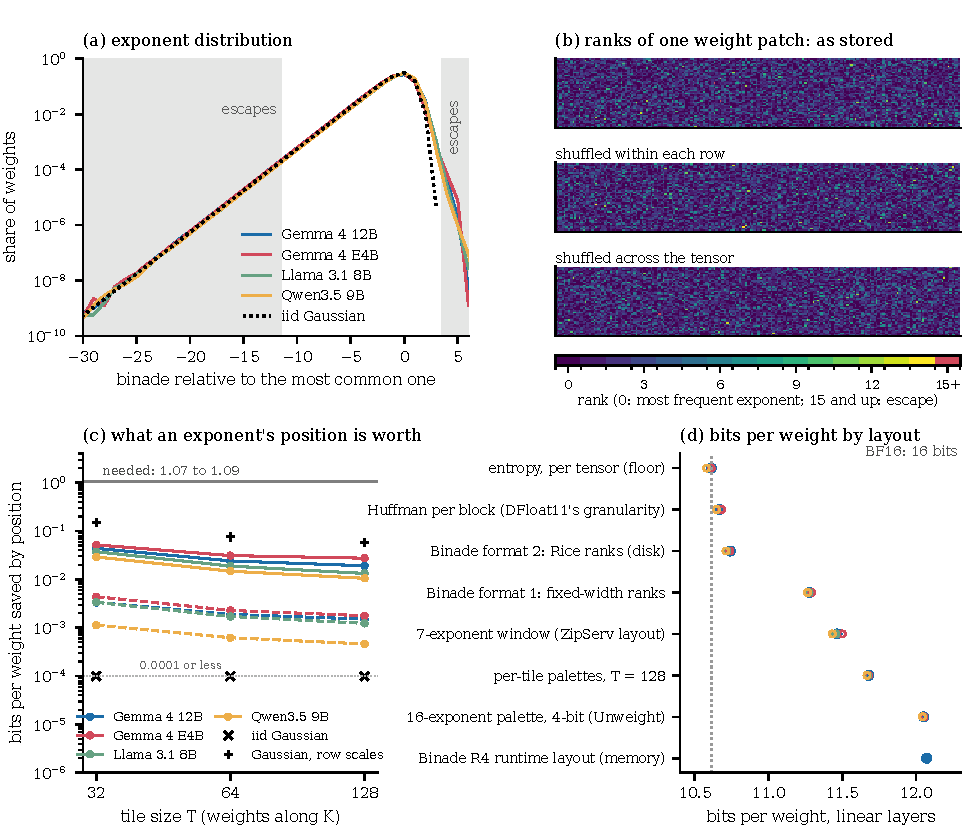
\includegraphics[width=\linewidth]{figures/stats.pdf}
\caption{The statistical basis of the format. (a) Share of linear-layer weights per binade, each model aligned at its most common binade, against iid Gaussian weights (scale averaged over one binade); shaded: binades outside the 15 most frequent of Gemma 4 12B's linear layers taken together, the region R4 stores as escapes (with ranks taken per tensor, 0.026\% of that model's weights). (b) Per-tensor frequency ranks of the exponents of a $48 \times 192$ corner of Gemma 4 12B's layer-20 gate projection, as stored, with each row's weights shuffled along K, and drawn from the whole tensor. (c) Bits per weight a per-tile palette code saves by keeping positions (its cost after shuffling minus its cost as stored, best of the tile codes), against the gap to per-tensor entropy coding that locality would have had to close; Gaussian models tiled the same way. (d) Bits per weight of the linear layers in each layout, all four models (Gemma 4 12B filled); every layout includes the 8-bit raw byte, and the dotted line is the per-tensor entropy.}
\label{fig:stats}
\end{figure}

Exponents concentrate on a few binades, and their distribution has the shape iid Gaussian weights would give it (Figure~\ref{fig:stats}a): the share of weights halves with each binade below the most common one, and only the largest weights fall off more slowly than a Gaussian's. Their entropy is 2.58 to 2.61 bits per weight (Table~\ref{tab:mi}). A fixed-width code with escapes for rare values spends 3.3 bits per exponent (format 1, Section~\ref{sec:format}); an entropy code needs about 2.6. Our starting hypothesis was that fixed-width codes could close most of that gap if exponents clustered along the reduction dimension K: a small tile would then hold few distinct values and need few index bits.

\paragraph{Locality test.} We cut every linear weight into tiles of $T=128$ consecutive weights along K and gave each tile its own palette (best of a direct index, an escape to a side stream, and verbatim storage, plus an 8-bit meta byte per tile). We then recomputed the cost after shuffling the exponents within each row, and within the whole tensor, which keeps the distribution and destroys any positional structure. Table~\ref{tab:locality} and Figure~\ref{fig:stats}c show the result for four models: shuffling the tensor raises the cost by only 0.011 to 0.027 bits per weight, and shuffling within rows by at most 0.002, against the 1.07 to 1.09 bits a palette code would need to gain to match entropy coding. A stored patch of exponents and the same weights shuffled look alike (Figure~\ref{fig:stats}b). The order of weights along K carries no exploitable exponent information, and per-tile palettes cost about 1 bit per weight more than Huffman coding because the palette itself is paid per tile.

\begin{table}[t]
\centering
\caption{Per-tile palette cost in bits per weight (linear layers, $T=128$), on real and shuffled exponents.}
\label{tab:locality}
\begin{tabular}{lrrrrr}
\toprule
model & linear weights & per-tile best-of & row-shuffled & tensor-shuffled & gain \\
\midrule
Gemma 4 12B & 10.90B & 11.679 & 11.680 & 11.698 & 0.019 \\
Gemma 4 E4B & 4.03B & 11.677 & 11.679 & 11.704 & 0.027 \\
Llama 3.1 8B & 6.98B & 11.672 & 11.673 & 11.685 & 0.013 \\
Qwen3.5 9B & 7.12B & 11.667 & 11.667 & 11.677 & 0.011 \\
\bottomrule
\end{tabular}

\end{table}

\paragraph{Reordering bound.} A search over column permutations or tile boundaries can only exploit statistical dependence between an exponent and its position. Table~\ref{tab:mi} gives the mutual information between the exponent $E$ and the row index $R$ or column index $C$ (Miller--Madow corrected). Any code whose statistics depend only on the column group has expected length at least $H(E \mid C)$, so it saves at most $I(E;C) \le 0.020$ bits per exponent.

\begin{table}[t]
\centering
\caption{Exponent entropy and its mutual information with the row and column index, bits per exponent.}
\label{tab:mi}
\begin{tabular}{lrrr}
\toprule
model & $H(E)$ & $I(E;R)$ & $I(E;C)$ \\
\midrule
Gemma 4 12B & 2.6110 & 0.0308 & 0.0167 \\
Gemma 4 E4B & 2.6113 & 0.0334 & 0.0197 \\
Llama 3.1 8B & 2.5822 & 0.0239 & 0.0087 \\
Qwen3.5 9B & 2.5806 & 0.0187 & 0.0087 \\
\bottomrule
\end{tabular}

\end{table}

\paragraph{The iid model.} Drawing weights iid from a Gaussian reproduces these costs without any structure: an exponent entropy of 2.545 bits and a per-tile best-of cost of 11.640 bits at $T=128$, with zero locality gain, against 11.667 to 11.679 on the real models. Adding a log-normal per-row scale ($\sigma = 0.3$) produces a gain of 0.058, more than any real model shows. For exponent coding, trained weights behave like unstructured draws (Figure~\ref{fig:stats}a, c).

\section{Format}
\label{sec:format}

The statistics point to per-tensor coding. Binade keeps one table per tensor listing its exponents by descending frequency, and stores each weight's rank instead of its exponent.

\paragraph{Format 1: fixed width with escapes.} Each 128-weight tile stores ranks at a width $b$ given in a meta byte: either $b$ equal to the bit length of the tile's largest rank, or $b \le 4$ with ranks of $2^b-1$ and above escaping to a per-tensor byte stream. No offsets are stored; they are derived at load. The cost is 11.27 to 11.29 bits per weight.

\paragraph{Format 2: Rice codes.} Each tile's ranks are Rice coded with a parameter $k \in \{0,\dots,3\}$ chosen per tile: a plane of $k$ low bits per weight, then unary bit planes, where plane $j$ holds one bit for every weight whose quotient is at least $j$. A tile costs $nk + \sum_i \min(q_i+1, q_{\max})$ bits, rows start on a 32-bit word, and a per-row word offset lets rows decode independently. Table~\ref{tab:sizes} and Figure~\ref{fig:stats}d compare the codes with baselines computed by the same scanner on the same tensors, and Table~\ref{tab:files} gives the packed checkpoints.

\begin{table}[t]
\centering
\caption{Bits per weight of exponent codes on the linear layers (raw byte included). Baselines are our accounting of each layout on the same tensors.}
\label{tab:sizes}
\resizebox{\linewidth}{!}{\begin{tabular}{lrrrrrrr}
\toprule
model & entropy & Huffman (block) & Rice ranks & fixed ranks & tile palettes & 7-exp. window & 16-palette, 4-bit \\
\midrule
Gemma 4 12B & 10.611 & 10.666 & 10.740 & 11.276 & 11.679 & 11.464 & 12.051 \\
Gemma 4 E4B & 10.611 & 10.680 & 10.737 & 11.292 & 11.677 & 11.501 & 12.054 \\
Llama 3.1 8B & 10.582 & 10.648 & 10.716 & 11.274 & 11.672 & 11.455 & 12.044 \\
Qwen3.5 9B & 10.581 & 10.646 & 10.711 & 11.265 & 11.667 & 11.432 & 12.043 \\
\bottomrule
\end{tabular}
}
\end{table}

\begin{table}[t]
\centering
\caption{Checkpoints in format 2, with a bit-exact round trip of every tensor.}
\label{tab:files}
\begin{tabular}{lrrrrrr}
\toprule
model & BF16 GB & Binade GB & ratio & bits/weight & tensors & mismatches \\
\midrule
Gemma 4 12B & 23.92 & 16.10 & 67.3\% & 10.746 & 677 & 0 \\
Llama 3.1 8B & 16.06 & 10.77 & 67.0\% & 10.726 & 291 & 0 \\
Qwen3.5 9B & 19.31 & 13.27 & 68.7\% & 10.722 & 775 & 0 \\
Gemma 4 26B-A4B & 51.61 & 35.05 & 67.9\% & 10.747 & 1013 & 0 \\
\bottomrule
\end{tabular}

\end{table}

\paragraph{Runtime layout.} A code is not a good layout for a matrix-vector kernel. In format 1 read in place, 83.5\% of tiles use the escape, and every escaped exponent's address depends on the tile's decoded codes; that dependent load caps the kernel at 72.6\% of BF16's bandwidth efficiency, and replacing it with a constant lifts efficiency to 84 to 90\%. Rice's plane-by-plane decode is a chain of such loads. Binade therefore separates the file from the runtime layout: at load, a GPU kernel transcodes either format into R4, which stores every rank in 4 bits (four per lane in one 16-bit word, in the lane order of the matrix-vector kernel) and escapes only ranks of 15 and above, 0.026\% of weights in 3.1\% of tiles. R4 takes 12.07 bits per weight in memory. All of its addresses except an escape's are known in advance, so the kernel prefetches two tiles ahead.

\section{Exact kernels}
\label{sec:kernels}

A kernel's output depends on the order in which it accumulates products, and every MLX kernel fixes that order through its thread layout and loop structure. Binade's kernels reproduce it.

\paragraph{Matrix-vector product.} MLX's batch-one kernel assigns a SIMD group to each output row; lane $i$ owns weights $4i$ to $4i+3$ of every 128-weight block along K, accumulates their products in float in K order, and a shuffle-down tree reduces the 32 partial sums. A Binade tile is exactly one such block, so the R4 kernel decodes a tile in registers and runs the same accumulation. When K is not a multiple of 128, MLX's last block adds $0 \times 0$ on idle lanes, and so does Binade. MLX switches to other layouts for $K \le 64$ (four lanes per row) and $K \ge 16N$ (K split across eight SIMD groups); there the runtime rebuilds the weight and calls MLX.

\paragraph{Mixture of experts.} mlx-lm evaluates experts with \texttt{gather\_mm}. For fewer than 64 expert slots, every decoding step, MLX runs one matrix-vector product per (token, expert) slot with the same per-row order, which a gather variant of the R4 kernel reproduces, gate and up rows in one launch.

\paragraph{GEMM.} MLX's tiled GEMM, and its gather variant over slots sorted by expert, accumulate every output element in float $8 \times 8 \times 8$ \texttt{simdgroup\_multiply\_accumulate} steps along K, in order, whatever their tile sizes, provided K is a multiple of the 16-element K block and the dispatcher does not split K. The R4 GEMM runs the same steps with the same fragment layout, so its tiling is a free choice. Like MLX's, it is register-blocked: in a $64 \times 64$ threadgroup tile each of four SIMD groups owns $32 \times 32$ outputs. It walks K in chunks of 32 inside each R4 tile: the chunk's inputs are staged in threadgroup memory while two threads per weight row decode 16 weights each, with the row's running escape pointer held in registers and escape counts read from the code nibbles. Staging chunks rather than whole R4 tiles keeps threadgroup memory near MLX's, so several threadgroups share a GPU core and hide one another's decoding. Expert segments are handled as in MLX's gather kernel, and smaller tiles serve short inputs. The runtime picks, per call and among exact paths only: the matrix-vector kernel for one row; the fused GEMM for up to 128 rows, or whenever rebuilding a BF16 weight would crowd GPU memory; otherwise the rebuilt weight and MLX's own matmul. The dispatch conditions follow MLX 0.32.2.

\paragraph{Testing exactness.} Random test data is weak evidence that a kernel reproduces a summation order: differences in a float accumulator almost never survive rounding the output to BF16. Our tests add rows of $2^{25}$, ones that vanish against it, and $-2^{25}$. Summed in order the result is 0; any other grouping keeps some of the ones, which BF16 represents exactly. A control case confirms the data's power: at $K=520$, MLX's GEMM adds the partial last K block first, and the in-order kernel then disagrees. This data found a real gap in our first matrix-vector dispatch rule, for the $K \ge 16N$ case above; no Gemma shape falls there.

\paragraph{CUDA, and a closed library.} MLX's CUDA backend computes the single-row product with one warp per row, thread $t$ owning $n$ consecutive weights of every block of $32n$ (with $n$ = 4, 2 or 1 depending on K), then \texttt{cooperative\_groups::reduce}. The CUDA kernels mirror this structure and call the same reduction. Every product with more than one row, including batched decoding, goes to cuBLASLt, which is closed. Its BF16 GEMM turned out to be reproducible all the same. Without split-K, each output is a sequence of tensor-core \texttt{mma.sync m16n8k16} steps along K, in order, from zero, then one rounding to BF16, whichever kernel cuBLAS picks: a plain kernel issuing the same instruction in the same order is bit-identical to six CUTLASS-derived kernels with different tiles that cuBLAS chose for the 12B's shapes. With split-K into $S$ partitions, the partitions are $\lceil K/S \rceil$ rounded up to a multiple of 64 (trailing ones may be empty); each is summed the same way and rounded to BF16 (reduction scheme \texttt{OUTPUT\_TYPE}) or kept in float32 (\texttt{COMPUTE\_TYPE}), and the partials are added in float32 in partition order; with the \texttt{INPLACE} scheme, chosen for long inputs, partition $s$ instead adds its float32 sum to the BF16 output left by partitions $0..s-1$ and rounds again. The algorithm for a given shape depends on the GPU (one algorithm family on the RTX PRO 6000, four on an L4, three on an A100), and on the A100 and the L4 one of them is sliced-K: its outputs are summed in two accumulators over alternating 32-wide slices of K and added at the end. $S$, the scheme and the algorithm are cuBLASLt's own choice per shape, which the runtime reads through the library's interface from the descriptors MLX builds (\texttt{cublasLtMatmulAlgoGetHeuristic}, then the algorithm's identifier, split-K and reduction attributes); the query reproduced every split count we observed with Nsight. A fused R4 tensor-core GEMM that follows this plan is bit-identical to cuBLAS on order-sensitive data for every shape and row count tested, on an RTX PRO 6000, an L4 and an A100: up to 64 input rows it decodes weights straight into the MMA's register fragments, and beyond that it stages decoded 128-row tiles in shared memory. For an algorithm or plan it has not measured, the runtime rebuilds BF16 weights for cuBLAS itself. Mixture-of-experts prompts run an open CUTLASS grouped GEMM in MLX (per expert, m16n8k16 steps along K in order, no split-K), which a gather variant of the fused kernel reproduces: slots sorted by expert are taken in tiles, and each run of one expert walks K with that expert's weights.

\section{Implementation}

Binade integrates with mlx-lm without patching it: the loader runs the model's own weight sanitizer on placeholders to find the module behind each packed weight, swaps those modules, and loads with strict shape checks. The packer streams a checkpoint one tensor at a time; the same input produces byte-identical files on Apple Silicon and on x86. For a model too large to hold in BF16, the exactness check needs a reference that fits: we load the stock model lazily and make each decoder layer read its weights from the checkpoint when it runs and release them after. Near the GPU's working-set limit, allocation and paging dominated our first prompt path; the runtime therefore wires GPU memory at load and avoids per-layer temporaries.

\section{Evaluation}
\label{sec:eval}

All Apple Silicon measurements use an M4 Max (40-core GPU, 546\,GB/s, 48\,GB) with MLX 0.32.2 and mlx-lm 0.31.3. Models: Gemma 4 12B, E4B and 26B-A4B, Llama 3.1 8B and Qwen3.5 9B, instruction-tuned BF16 checkpoints with verified hashes. Every number comes from a script in the repository.

\paragraph{Exactness at scale.} For each model we compute the logits at every position of 32 windows of 512 tokens from the WikiText-2 test set in one forward pass (exercising the multi-row paths), and greedily decode 128 tokens from 32 prompts (the single-row paths). Table~\ref{tab:exact} compares Binade and MLX's 8-bit affine quantization against BF16. Binade's logits are bit-identical at all 16,352 positions for every model, and all generations match token for token with identical log-probabilities. 8-bit quantization matches at no position and in no generation; its greedy argmax disagrees with BF16 at 1.8 to 15\% of positions. Forcing the fused GEMM onto the 512-token windows, the path a model without memory headroom takes, is equally exact. Gemma 4 26B-A4B takes that path: against a BF16 reference whose decoder layers are read from disk as they run, all 16,352 of its positions are bit-identical, while 8-bit quantization agrees with BF16's argmax at only 76.4\% of them. To measure what this exactness protects against, we also ran Binade with one change a kernel writer might make for speed: every kernel sums even and odd K steps in two accumulators and adds them at the end. That is a valid order with two independent dependency chains, but not MLX's; the weights and every product are unchanged, and our order-sensitive tests flag it. On Llama 3.1 8B no position keeps bit-identical logits, the argmax changes at 1.2\% of positions and no generation survives 128 tokens unchanged; on Gemma 4 12B the argmax changes at 11.5\% of positions, close to 8-bit quantization's 15\%, and perplexity moves from 729.4 to 754.4.

\begin{table}[t]
\centering
\caption{Exactness against BF16 on WikiText-2 (32 windows of 512 tokens) and 32 greedy generations of 128 tokens. Binade, fused GEMM: the fused GEMM forced onto every prompt length. Two accumulators: the order ablation. $^\dagger$Windows only, against BF16 layers streamed from disk, since BF16 does not fit in memory.}
\label{tab:exact}
\resizebox{\linewidth}{!}{\begin{tabular}{llrrrrr}
\toprule
model & variant & identical logits & argmax agr. & perplexity (BF16) & identical gen. & identical tokens \\
\midrule
Gemma 4 12B & Binade & 16,352 / 16,352 & 100.0\% & 729.42 (729.42) & 32 / 32 & 100.0\% \\
 & Binade, fused GEMM & 16,352 / 16,352 & 100.0\% & 729.42 (729.42) & 32 / 32 & 100.0\% \\
 & two accumulators & 0 / 16,352 & 88.5\% & 754.35 (729.42) & 0 / 32 & 37.8\% \\
 & 8-bit & 0 / 16,352 & 85.0\% & 739.13 (729.42) & 0 / 32 & 30.5\% \\
Gemma 4 E4B & Binade & 16,352 / 16,352 & 100.0\% & 76.41 (76.41) & 32 / 32 & 100.0\% \\
 & Binade, fused GEMM & 16,352 / 16,352 & 100.0\% & 76.41 (76.41) & 32 / 32 & 100.0\% \\
 & 8-bit & 0 / 16,352 & 96.4\% & 75.70 (76.41) & 0 / 32 & 34.4\% \\
Llama 3.1 8B & Binade & 16,352 / 16,352 & 100.0\% & 8.89 (8.89) & 32 / 32 & 100.0\% \\
 & Binade, fused GEMM & 16,352 / 16,352 & 100.0\% & 8.89 (8.89) & 32 / 32 & 100.0\% \\
 & two accumulators & 0 / 16,352 & 98.8\% & 8.89 (8.89) & 0 / 32 & 62.4\% \\
 & 8-bit & 0 / 16,352 & 98.2\% & 8.89 (8.89) & 0 / 32 & 34.6\% \\
Qwen3.5 9B & Binade & 16,352 / 16,352 & 100.0\% & 8.56 (8.56) & 32 / 32 & 100.0\% \\
 & Binade, fused GEMM & 16,352 / 16,352 & 100.0\% & 8.56 (8.56) & 32 / 32 & 100.0\% \\
 & 8-bit & 0 / 16,352 & 98.2\% & 8.55 (8.56) & 0 / 32 & 53.3\% \\
Gemma 4 26B-A4B$^\dagger$ & Binade & 16,352 / 16,352 & 100.0\% & 16782.18 (16782.18) & n/a & n/a \\
 & 8-bit & 0 / 16,352 & 76.4\% & 16998.88 (16782.18) & n/a & n/a \\
\bottomrule
\end{tabular}
}
\end{table}

Exactness is defined against MLX's BF16 run of each model, so that run must itself be the model. Gemma 4 12B is a model type mlx-lm lacks, which our loader maps to mlx-lm's Gemma 4 implementation. Table~\ref{tab:reference} compares MLX with the reference implementation (Hugging Face transformers) on the same 512 tokens. In float32, where two implementations of one function differ only by rounding, the per-token losses agree to 0.0002 to 0.015 nats on average and the argmax at 99.4 to 99.8\% of positions on all three models. In BF16 the same two implementations drift apart: the argmax agrees at 98.8\% of positions on E4B, 94.1\% on the 12B and only 74.6\% on the mixture-of-experts 26B-A4B, where a rounding difference in the router selects different experts. Rounding differences that are harmless in float32 change a quarter of the BF16 MoE model's next-token predictions, which is why we define exactness at the bit level rather than by closeness. The Gemma models' high perplexities on raw text are a property of the instruction-tuned checkpoints, reproduced by the reference implementation.

\begin{table}[t]
\centering
\caption{MLX against the reference implementation on 512 WikiText-2 tokens, both sides on the same device (the 26B in float32 does not fit the GPU and ran on the CPU): perplexity, argmax agreement and per-token loss difference in nats.}
\label{tab:reference}
\begin{tabular}{lllrrrr}
\toprule
model & dtype & device & perplexity (ref. / MLX) & argmax agr. & mean $|\Delta|$ & max $|\Delta|$ \\
\midrule
Gemma 4 E4B (native) & float32 & CUDA & 43.22 / 43.22 & 99.80\% & 0.0020 & 0.043 \\
 & bfloat16 & CUDA & 43.40 / 43.21 & 98.83\% & 0.0725 & 1.380 \\
Gemma 4 12B (aliased) & float32 & CUDA & 715.20 / 713.03 & 99.41\% & 0.0145 & 0.880 \\
 & bfloat16 & CUDA & 725.75 / 724.33 & 94.13\% & 0.2298 & 7.881 \\
Gemma 4 26B-A4B (native) & float32 & CPU & 6631.63 / 6630.75 & 99.80\% & 0.0002 & 0.005 \\
 & bfloat16 & CUDA & 6085.05 / 7504.68 & 74.56\% & 1.1374 & 17.808 \\
\bottomrule
\end{tabular}

\end{table}

\paragraph{Decoding speed.} Table~\ref{tab:decode} gives greedy decoding speed, the median of three fresh processes per model, 256 tokens after a 16-token warm-up. Binade decodes 1.25 to 1.35\x{} faster than BF16 with identical tokens; 8-bit quantization, which changes the outputs, is 1.78 to 1.83\x{} faster. Gemma 4 26B-A4B has no BF16 entry: its checkpoint does not load. Binade runs it in 35\,GB, and with the BF16 reference streamed layer by layer from disk its prompt logits and 64 greedy tokens are identical to BF16.

\begin{table}[t]
\centering
\caption{Greedy decoding, tokens per second (median of three fresh processes).}
\label{tab:decode}
\begin{tabular}{lrrrrr}
\toprule
model & BF16 & Binade & 8-bit & Binade/BF16 & 8-bit/BF16 \\
\midrule
Gemma 4 12B & 19.2 & 24.7 & 35.0 & 1.29$\times$ & 1.83$\times$ \\
Gemma 4 E4B & 42.2 & 52.6 & 75.0 & 1.25$\times$ & 1.78$\times$ \\
Llama 3.1 8B & 28.4 & 38.3 & 50.7 & 1.35$\times$ & 1.78$\times$ \\
Qwen3.5 9B & 26.9 & 34.4 & 48.7 & 1.28$\times$ & 1.81$\times$ \\
Gemma 4 26B-A4B & n/a & 58.8 & 77.0 & n/a & n/a \\
\bottomrule
\end{tabular}

\end{table}

\paragraph{Kernel efficiency.} Table~\ref{tab:kernel} isolates the batch-one matrix-vector products of Gemma 4 12B, streamed from DRAM. The R4 kernel reads 0.755 of BF16's bytes at BF16's bandwidth efficiency, 1.33\x{} per token. Without prefetching, isolated products already ran at 1.31\x{} but whole-model decoding reached only 1.19\x{}: a decoding step is a chain of dependent products, which exposes each launch's tail.

\begin{table}[t]
\centering
\caption{Batch-one matrix-vector products of Gemma 4 12B, per token (every projection once plus the output layer).}
\label{tab:kernel}
\begin{tabular}{llrrrrr}
\toprule
GPU & method & ms/token & bytes & GB/s & efficiency & speedup \\
\midrule
M4 Max (Metal) & BF16 & 48.2 & 1.000 & 494 & 100.0\% & 1.00$\times$ \\
 & 8-bit (lossy) & 25.7 & 0.531 & 491 & 99.4\% & 1.87$\times$ \\
 & format 1 in place & 47.3 & 0.712 & 359 & 72.6\% & 1.02$\times$ \\
 & R4 & 36.2 & 0.755 & 496 & 100.3\% & 1.33$\times$ \\
RTX PRO 6000 (CUDA) & BF16 & 15.3 & 1.000 & 1553 & 100.0\% & 1.00$\times$ \\
 & 8-bit (lossy) & 8.7 & 0.531 & 1462 & 94.1\% & 1.77$\times$ \\
 & R4 & 13.5 & 0.755 & 1333 & 85.8\% & 1.14$\times$ \\
\bottomrule
\end{tabular}

\end{table}

\paragraph{Prompt processing.} Prompts are compute-bound, so a fused decode must keep pace with MLX's GEMM rather than with memory. Figure~\ref{fig:prefill} shows the matrix products of a Gemma 4 12B prompt pass. The runtime is 1.30\x{} BF16 for 16 prompt rows, 0.77 to 0.90\x{} for 32 to 128, and 0.89 to 0.95\x{} for 512 to 2048 rows, where it rebuilds weights; BF16's own 16-row GEMM varied by up to 20\% between runs on this machine, so the 16-row figure is approximate. On long prompts the fused GEMM runs at 0.75\x{} of MLX's BF16 GEMM (4.6 against 3.5\,s of matrix products at 2048 rows), which is what a model without memory headroom pays; our first version, which decoded whole 128-weight R4 tiles into $32 \times 32$ threadgroup tiles, reached 0.37 to 0.42\x{}. Ablations place the remaining gap: the MMA steps alone run as fast as MLX's whole GEMM, and the decoding and input staging before each chunk are not fully hidden. Keeping the next chunk's loads in registers (software pipelining) was slower, because the extra registers and buffers reduce occupancy. Gemma 4 26B-A4B, which has no memory headroom and runs the fused GEMM at every prompt length, reaches its first token 0.32\,s after a 40-token prompt and 2.0\,s after a 2048-token one, with prompt logits identical to the streamed BF16 reference.

\begin{figure}[tbp]
\centering
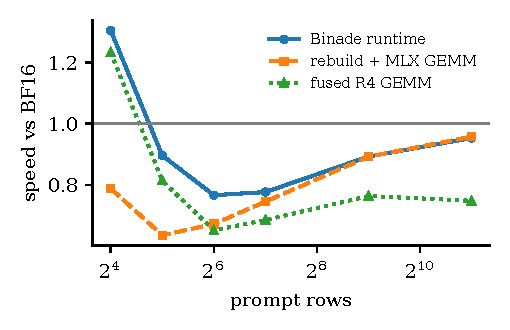
\includegraphics[width=0.48\linewidth]{figures/prefill.pdf}
\caption{Matrix products of a Gemma 4 12B prompt pass, speed relative to BF16.}
\label{fig:prefill}
\end{figure}

\paragraph{CUDA.} On an NVIDIA RTX PRO 6000 Blackwell (96\,GB), the runtime on MLX's CUDA backend is bit-identical to BF16 on five models at every WikiText-2 position and in every generation of the test above, where 8-bit quantization matches none (Table~\ref{tab:exactcuda}). Decoding is bound by the GPU for the dense models and runs 1.05 to 1.10\x{} faster than BF16 with 20 to 25\% less memory; it is limited on medium-sized matrices, where one warp per row exposes too little parallelism and splitting a row's reduction would change its order. The 26B mixture-of-experts model decodes at 1.01\x{}: injecting CPU work after each token lengthened its step one for one, so the step is bound by the CPU's construction of the graph; removing reshape, cast and slice nodes from every kernel call raised it from 0.95\x{}. Fusing query, key and value into one launch was slower, because MLX's CUDA graphs already overlap the separate kernels.

\begin{table}[t]
\centering
\caption{CUDA (RTX PRO 6000): exactness against resident BF16 (test of Table~\ref{tab:exact}), 8-bit for reference, decoding speed and peak memory.}
\label{tab:exactcuda}
\resizebox{\linewidth}{!}{\begin{tabular}{lrrrrrr}
\toprule
model & identical logits & identical gen. & 8-bit ident. & 8-bit argmax & decode vs BF16 & peak GB (BF16) \\
\midrule
Llama 3.1 8B & 16,352 / 16,352 & 32 / 32 & 0 & 98.1\% & 1.05$\times$ & 14.4 / 16.2 \\
Qwen3.5 9B & 16,352 / 16,352 & 32 / 32 & 0 & 98.1\% & 1.10$\times$ & 16.5 / 18.4 \\
Gemma 4 12B & 16,352 / 16,352 & 32 / 32 & 0 & 85.0\% & 1.06$\times$ & 20.0 / 24.1 \\
Gemma 4 26B-A4B & 16,352 / 16,352 & 32 / 32 & 0 & 77.2\% & 1.01$\times$ & 40.0 / 51.9 \\
Gemma 4 31B & 16,352 / 16,352 & 32 / 32 & 0 & 89.4\% & 1.10$\times$ & 49.2 / 62.1 \\
\bottomrule
\end{tabular}
}
\end{table}

On GPUs too small for the BF16 checkpoint, BF16 fails with out-of-memory while Binade runs, with logits identical to a BF16 reference streamed from disk at all 16,352 positions and identical generation (Table~\ref{tab:fitcuda}): Gemma 4 12B on a 24\,GB L4 and Gemma 4 26B-A4B on a 40\,GB A100. Exact BF16 inference on hardware that cannot hold BF16 is, on CUDA as on the Mac, the clearest use of lossless compression.

\begin{table}[t]
\centering
\caption{Smaller NVIDIA GPUs: BF16 does not load; Binade against BF16 decoder layers streamed from disk (32 windows of 512 tokens).}
\label{tab:fitcuda}
\resizebox{\linewidth}{!}{\begin{tabular}{llllrl}
\toprule
GPU & model & BF16 & Binade: peak, decode & identical logits (fused forced) & 8-bit: peak, decode \\
\midrule
L4 (24.2\,GB) & Gemma 4 12B & out of memory & 20.0\,GB, 11.1 tok/s & 16,352 / 16,352 (16,352) & 14.7\,GB, 17.9 tok/s \\
A100 40\,GB (42.9\,GB) & Gemma 4 26B-A4B & out of memory & 40.0\,GB, 46.5 tok/s & 16,352 / 16,352 (16,352) & 28.3\,GB, 55.2 tok/s \\
\bottomrule
\end{tabular}
}
\end{table}

Prompts are the weak spot on CUDA. Rebuilding BF16 weights for cuBLAS moves about 5.5 bytes per weight against BF16's 2: the first token after a 40-token prompt took 77\,ms for Gemma 4 12B (BF16: 45\,ms) and 117\,ms for the 26B mixture-of-experts model (BF16: 42\,ms), which rebuilt all its experts for every prompt. Product by product, the fused GEMMs run at 0.63 to 0.81 of cuBLAS's speed from 40 to 512 rows on the 12B's weights (1.16 for one shape at 128 rows), where a rebuild runs at 0.21 to 0.69; only above about 1,000 rows does the rebuild catch up. A prompt pass is another matter: the rebuild's decoding does not depend on the activations, so it overlaps other layers' work, and it ties the fused kernel end to end beyond 128 rows. The runtime therefore uses the fused GEMMs for dense products up to 128 rows and for expert products at every length. On the RTX PRO 6000 the first token then comes after 59\,ms for the 12B and 53\,ms for the 26B at 40 tokens (BF16: 45 and 41\,ms), 72 and 66\,ms at 128 tokens (BF16: 47 and 52), and 0.100 and 0.088\,s at 512 tokens (BF16: 0.068 and 0.071), where 8-bit quantization's mixture-of-experts path takes 0.282\,s. With the fused GEMMs forced on every prompt length, both models keep all 16,352 positions and all 32 generations of the at-scale test identical. On the smaller GPUs, where BF16 does not load, the first token after 40 tokens went from 0.478 to 0.257\,s for the 12B on the L4 (8-bit: 0.148\,s) and from 0.252 to 0.101\,s for the 26B on the A100 (8-bit: 0.084\,s); from 128 tokens on, the 26B on the A100 answers sooner than with 8-bit quantization (0.123 against 0.169\,s at 128 tokens, 0.302 against 0.548\,s at 512). With the fused GEMMs forced on every length, the at-scale test stays identical on both cards.

\section{Discussion and limitations}
\label{sec:discussion}

The exponent's entropy caps lossless BF16 compression near 10.6 bits per weight, a 1.5\x{} reduction at best; 8-bit quantization goes further. The case for lossless compression is therefore exactness: evaluations that must reproduce a reference model, published checkpoints whose behavior must not change, and fitting an exact model into memory it would otherwise not fit. Our results show that exactness at the level of outputs is achievable without giving up the speed of fused decoding, but only by treating the framework's reduction order as part of the specification.

Exactness also constrains the design space. On CUDA, the R4 kernel reaches 90 to 97\% of BF16's efficiency on the largest matrices but 74 to 80\% on medium ones, where one warp per row exposes too little parallelism; the usual remedy, splitting a row's reduction across warps, changes the summation order and is therefore unavailable.

Exactness does not require the framework's kernels to be open. cuBLAS is closed, yet its BF16 GEMM follows a simple, recoverable order once the algorithm it chose is known, and the library reports that choice. Mirroring a closed library makes the claim depend on its version and on the GPU, so the plan has to be queried at run time and checked by tests on each GPU. The A100 showed why: the same split-K plan as on the RTX PRO 6000 came with a different algorithm for some shapes, which the order-sensitive tests caught. We have checked the fused CUDA GEMMs on an RTX PRO 6000, an L4 and an A100; on other GPUs the runtime rebuilds BF16 weights, which is exact but slower.

That specification is tied to a framework version and GPU generation: MLX 0.32.2, and for the fused GEMM, M3 and M4 GPUs. A new version can change the order; our tests detect it, and the runtime then needs updating. On CUDA, decoding runs at 1.01 to 1.10\x{} BF16's speed, and prompts still take longer than with BF16. Gemma E-models keep their per-layer embedding tables in BF16.

\section{Conclusion}

Exact weights do not imply exact outputs. Binade compresses BF16 weights losslessly to about 10.75 bits per weight on disk and runs them with kernels that reproduce the framework's floating-point reduction order, so five models produce outputs bit-identical to BF16 while decoding 1.25 to 1.35\x{} faster on Apple Silicon and 1.01 to 1.10\x{} on an NVIDIA GPU, and models that do not fit in BF16 run exactly on both. The same discipline extends to a closed library: cuBLAS's GEMM order can be read from the algorithm it reports and reproduced by a compressed kernel.

\bibliographystyle{plainnat}
\bibliography{refs}

\end{document}
